\documentclass{article}

\usepackage{circuitikz}
\usepackage[T1]{fontenc} 
\usepackage[UTF8]{inputenc}
\usepackage{amsmath}
\usepackage{amssymb}
\usepackage{fancyhdr}
\usepackage{graphicx}
\usepackage{hyperref}
\usepackage{tikz}
  \usetikzlibrary{arrows}
  \usetikzlibrary{shapes}
  \usetikzlibrary{arrows.meta,topaths}
  \usetikzlibrary{bending}
  \usetikzlibrary{calc}
\usepackage{anyfontsize}
\usepackage{sectsty}
\usepackage{../assets/scripts/tex/color-env}
\usepackage{anyfontsize}
\usepackage{xcolor}
\definecolor{DarkGreenBlue}{HTML}{264653}
\definecolor{LightGreenBlue}{HTML}{2A9D8F}
\definecolor{LightOrange}{HTML}{E9C46A}
\definecolor{DarkOrange}{HTML}{F4A261}
\definecolor{RedOrange}{HTML}{E76F51}
\definecolor{BrightRed}{HTML}{D62828}
\definecolor{DeepBlue}{HTML}{003049}



\usepackage[ngerman]{babel}
\title{Elektrotechnik 1 - Praktikum 3}


\usepackage[
  includehead,
  headheight = 17mm,
  footskip = \dimexpr\headsep+\ht\strutbox\relax,
  tmargin = 0mm,
  bmargin = \dimexpr17mm+2\ht\strutbox\relax,
]{geometry}





\pagestyle{fancy}
\fancyhead[L]{\leftmark}
\fancyhead[R]{}
\fancyfoot[L]{}
\fancyfoot[C]{\thepage}
\fancyfoot[R]{
\includegraphics[scale=0.2]{../assets/images/haw.jpg}}
\renewcommand\headrulewidth{0.5pt}

\begin{document}

\thispagestyle{empty}
\begin{tikzpicture}[remember picture,overlay]

  \fill[DeepBlue] (current page.south west) rectangle (current page.north east);

  \begin{scope}

    \foreach \i in {2.5,...,22}
      {
        \node[rounded corners, DeepBlue!90,draw ,regular polygon, regular polygon sides=6, minimum size=\i cm, ultra thick] at ($(current page.west)+(2.5,-5)$) {} ;
      }

  \end{scope}

  \node[rounded corners,fill=DeepBlue!95,text =DeepBlue!5,regular polygon,regular polygon sides=6, minimum size=2.5 cm,inner sep=0,ultra thick] at ($(current page.west)+(2.5,-5)$) {\LARGE \bfseries 2020};

  \foreach \i in {0.5,...,22}
    {
      \node[rounded corners,DeepBlue!90,draw,regular polygon,regular polygon sides=6, minimum size=\i cm,ultra thick] at ($(current page.north west)+(2.5,0)$) {} ;
    }

  \foreach \i in {0.5,...,22}
    {
      \node[rounded corners,DeepBlue!98,draw,regular polygon,regular polygon sides=6, minimum size=\i cm,ultra thick] at ($(current page.north east)+(0,-9.5)$) {} ;
    }

  \foreach \i in {12}
    {
      \node[fill = DeepBlue,rounded corners,draw=DeepBlue,regular polygon,regular polygon sides=6, minimum size=\i cm,ultra thick] at ($(current page.south east)+(-0.2,-0.45)$) {} ;
    }


  \foreach \i in {21,...,6}
    {
      \node[DeepBlue!95,rounded corners,draw,regular polygon,regular polygon sides=6, minimum size=\i cm,ultra thick] at ($(current page.south east)+(-0.2,-0.45)$) {} ;
    }

  \node[left,DeepBlue!5,minimum width=0.625*\paperwidth,minimum height=3cm, rounded corners] at ($(current page.north east)+(0,-9.5)$){{\fontsize{25}{30} \selectfont \bfseries ET2 - Praktikum 6}};

  \node[left,DeepBlue!10,minimum width=0.625*\paperwidth,minimum height=2cm, rounded corners] at ($(current page.north east)+(0,-11)$){{\huge \textit{Transiente Vorgänge}}};

  \node[left,DeepBlue!5,minimum width=0.625*\paperwidth,minimum height=2cm, rounded corners] at ($(current page.north east)+(0,-13)$){{\Large \textsc{Florian Tietjen\hspace{0.5cm}Eric Antosch}}};

\end{tikzpicture}

\newpage
\thispagestyle{empty}

\tableofcontents


\newpage

\section{Vorbereitung}
\subsection{Schaltvorgang einer RC-Reihenschaltung}

\subsection{Schaltvorgang bei einem Netzwerk mit einem Kondensator (ein Schaltzeitpunkt)}

\subsection{Schaltvorgang bei einem Netzwerk mit einem Kondensator (zwei Schaltzeitpunkte)}

\subsection{Funktion eines Tastteilers}
Ein Tastteiler, auch Prüfling oder Tastkopf genannt, ist ein Messmittel, welches am Oszilloskop angeschlossen wird. Dabei handelt es sich um ein Koaxialkabel, welches das Oszilloskop elektrisch sowie physisch mit der Signalquelle verbindet.
 
\subsection{Funktion und Aufbau eines Relais}
Ein Relais ist vereinfacht gesagt ein elektromagnetischer Schalter, welcher durch Anlegen einer Spannung seine Ein- und Ausgänge schließt oder öffnet.
 
\subsection{Funktion einer Freilaufdiode}
\begin{figure}[h]
  \begin{center}
    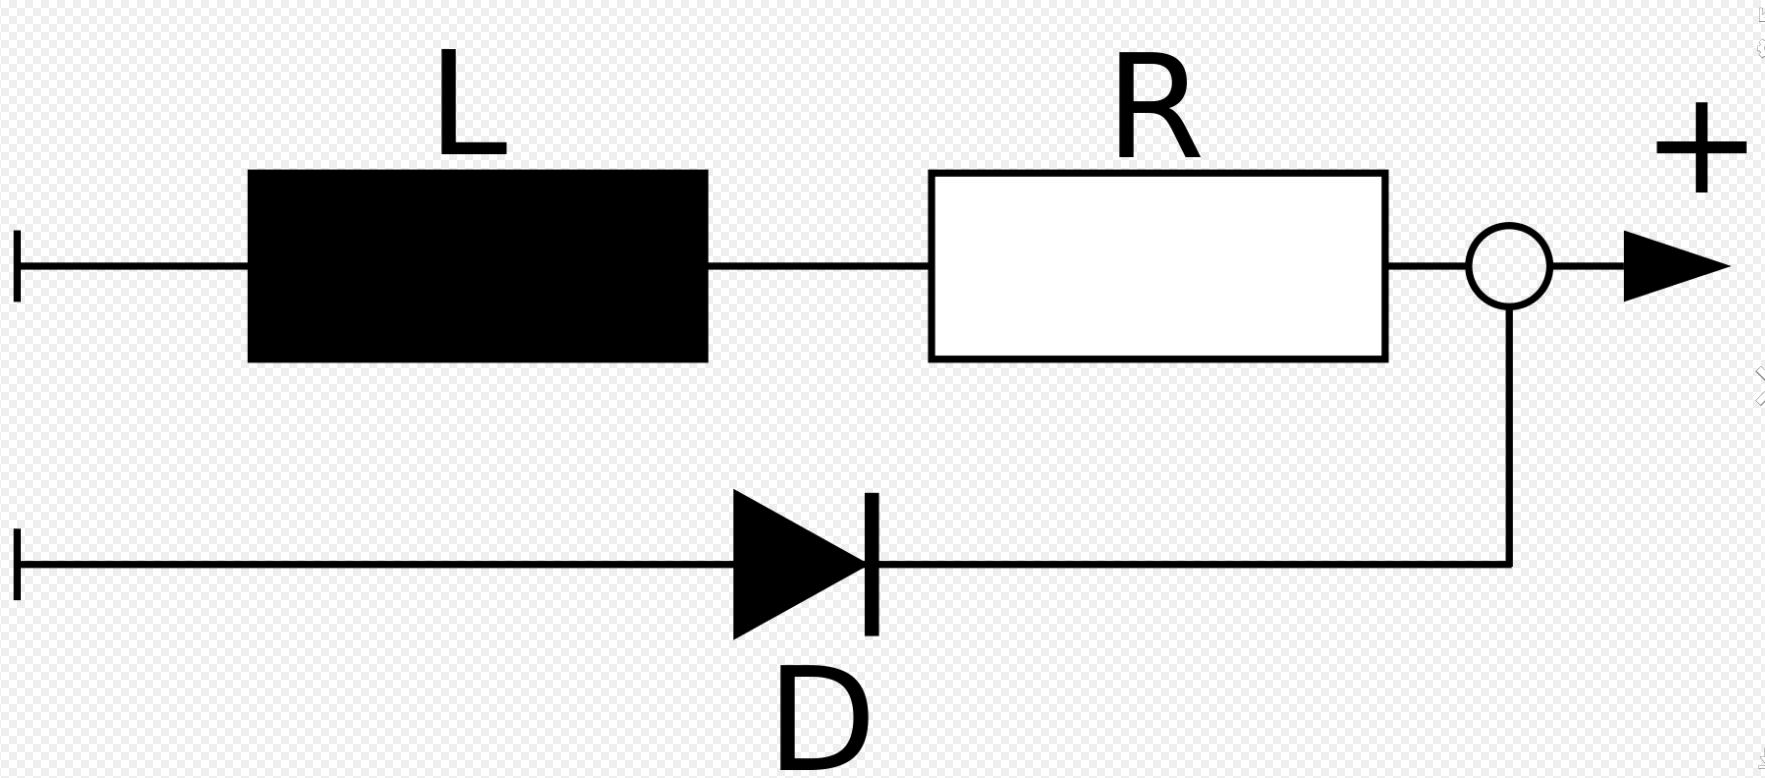
\includegraphics[scale=0.2]{../assets/images/ET2P4/freilaufdiode.JPG}
    \caption{Schaltung mit Freilaufdiode}
\end{center}
\end{figure}
Freilaufdioden sind Dioden, die zum Schutz vor Überspannung beim Abschalten einer induktiven Last dienen.
Nach dem Abschalten der Versorgungsspannung sorgt die Selbstinduktion einer Spule dafür, dass der Strom zunächst in der ursprünglichen Richtung weiter fließt. 
Ohne Freilaufdiode führt das zu einer Spannungsspitze, die sich zur Betriebsspannung addiert und dabei elektrische Bauteile beschädigen könnte.
Mit einer Freilaufdiode wird die Spannungsspitze jedoch auf die Durchlassspannung der Diode (bei Siliziumdioden etwa 0,7 V) begrenzt. 
\newpage

\section{Zeitmessung}

\begin{task}
    TIn dieser Aufgabe wollen wir den genauen Verlauf eines Rechtecksignals aus einem Funktionsgenerator analysieren.
\end{task}
\begin{devlist}
    T\begin{itemize}
        \item Oszilloskop Tektronix MDO3012
        \item Funktionsgenerator Rhode \& Schwarz HM8150
    \end{itemize}
\end{devlist}
Wir wollen nun zunächst die Anstiegs - und Abfallzeit bestimmen. Dazu messen wir die Zeit, die der Impuls benötigt, um von 10\%
vom absoluten Spannungsbodens bis zu 10\% vom absoluten Spannungsdach zu kommen. Diese Zeit nennen wir Anstiegszeit $t_{rise}=206,5\mu s $ . Gleichermaßen
messen wir die Zeit von 10\% vom absoluten Spannungsdach bis zu 10\% vom absoluten Spannungsboden. Diese Zeit nennen wir Abfallzeit $t_{fall} = 184\mu s$.

Mithilfe des Oszilloskops bestimmen wir nun die Frequenz $\mathrm{f} = 322,56Hz$ und das Tastverhältnis $\mathrm{a} = \frac{t_{high}}{T} = 58,06\%$.

\begin{figure}[h]
    \begin{center}
        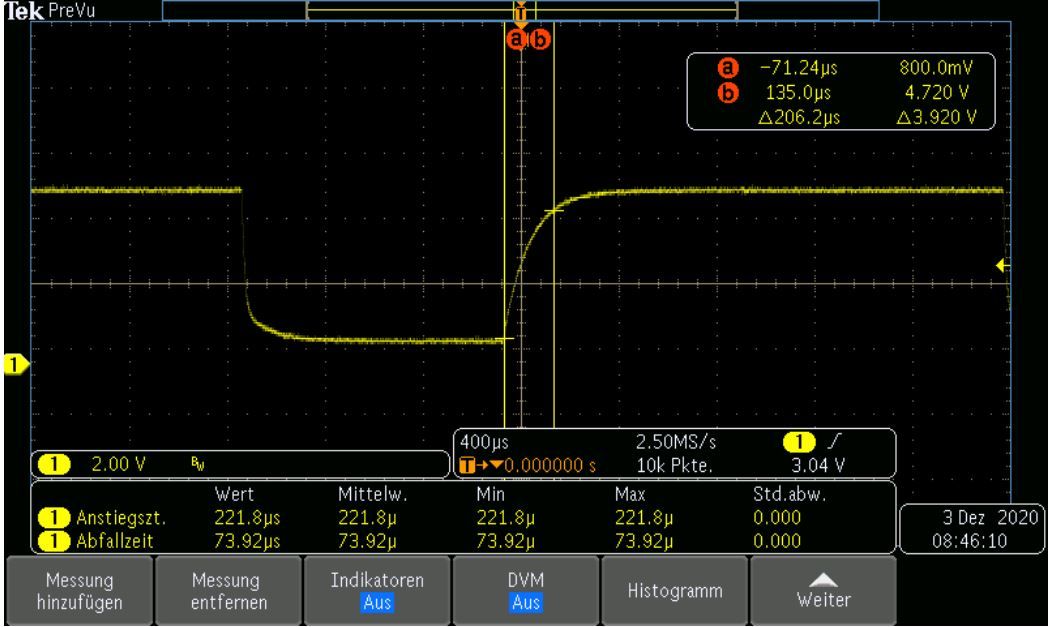
\includegraphics[scale=0.45]{../assets/images/ET2P4/aufgabe1.JPG}
        \caption{Oszilloskop-Bild der Rechteckspannung mit Cursorfunktion}
    \end{center}
\end{figure}

\newpage


\section{Einschalt- und Ausschaltvorgang an einem Relais}

\begin{task}
    TIn dieser Aufgabe wollen wir die Funktionsweise, sowie die entstehenden Spannungen und Ströme bei Schaltvorgängen mit Relais
    genauer analysieren. Dazu verwenden wir eine einfache Schaltung, die sich in Steuer- und Laststromkreis aufteilt. Der Shunt-Widerstand $R_M = 100\Omega$ dient als Messmittel
    zum Bestimmen der Ströme.
\end{task}
\begin{figure}[h]
    \begin{center}
        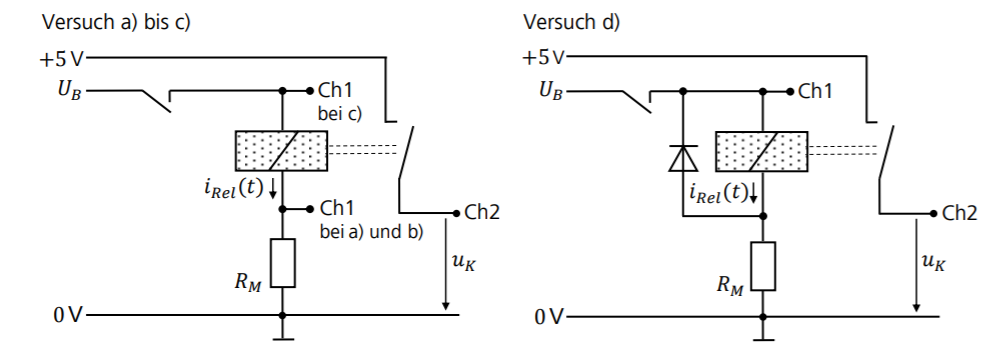
\includegraphics[scale=0.8]{../assets/images/ET2P4/Schaltplan2.PNG}
        \caption{Schaltplan des zweiten Versuchs mit eingezeichneten Aufnahmen der Messungen durch das Oszilloskop}
    \end{center}
\end{figure}



\begin{devlist}
    T\begin{itemize}
        \item Oszilloskop Tektronix MDO3012
        \item Funktionsgenerator Rhode \& Schwarz HM8150
        \item 1:10 Tastteiler
        \item Relais
        \item 1N4007 Freilaufdiode
        \item Multimeter MetraHit Tech
        \item Shuntwiderstand $100\Omega$
    \end{itemize}
\end{devlist}


\subsection{Verhalten des Relais im stationären Zustand}

Zunächst erhöhen wir von $U_B = 0V$ ausgehend die Spannung, bis wir das Relais zum Anzug bringen. Der entsprechende Strom $I_{an} = 7mA$ findet sich bei einer Spannung $U_{an} = 6,1V$; den Strom bezeichnen wir als 
den Anzugstrom; er stellt den minimalen Strom dar, der benötigt wird, damit das Relais anzieht.
Als nächstes wollen wir nun den Strom $I_{end} = 14,78mA$ herausfinden, welcher den Storm bei $U_B = 15V$ im stationären Zustand darstellt. Von diesem Punkt aus
reduzieren wir nun die Spannung wieder allmählich, bis das Relais erneut abfällt. Diesen Punkt bezeichnen wir als Abfallstrom $I_{ab} = 2,82mA$ bei einer Abfallspannung von $U_{ab} = 2,4V$.


\subsection{Einschaltvorgang}

Wir stellen nun mit dem Oszilloskop im Zweikanalbetrieb den Strom über den Shuntwiderstand $R_M$ und die Spannung $u_k$ über den Schaltkontakt dar.
Von besonderem Interesse ist hier dann die Verzögerungszeit $t_{ein} = 8,292ms$, die den zeitlichen Unterschied zwischen dem Einschalten der Versorgungsspannung des
Relais und des Umschalten des Relais darstellt.

\begin{figure}[h]
    \begin{center}
        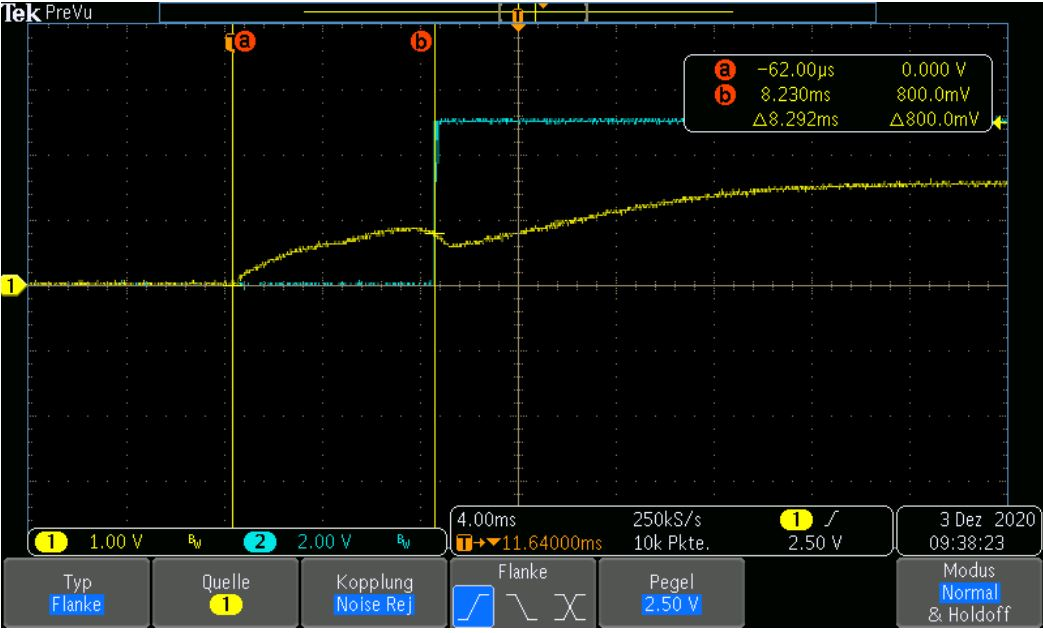
\includegraphics[scale=0.45]{../assets/images/ET2P4/aufgabe2b.JPG}
        \caption{Die Bestimmung des Einschaltvorgangs mit den entsprechenden Werten}
    \end{center}
\end{figure}

\subsection{Auschaltvorgang ungelöscht}

Ähnlich zum vorigen Versuch untersuchen wir nun hier den Ausschaltvorgang ohne Freilaufdiode, indem wir dem eingeschwungenem System nun die 
Versorgungsspannung entziehen. Dabei wollen wir die Maximalspannung $\hat{u}_{Rel} = 5,08V$ im Moment des Ausschalten des Relais messen, sowie die Ausschaltverzögerung
$t_{aus} = 3,283ms$.

\begin{figure}[!h]
    \begin{center}
        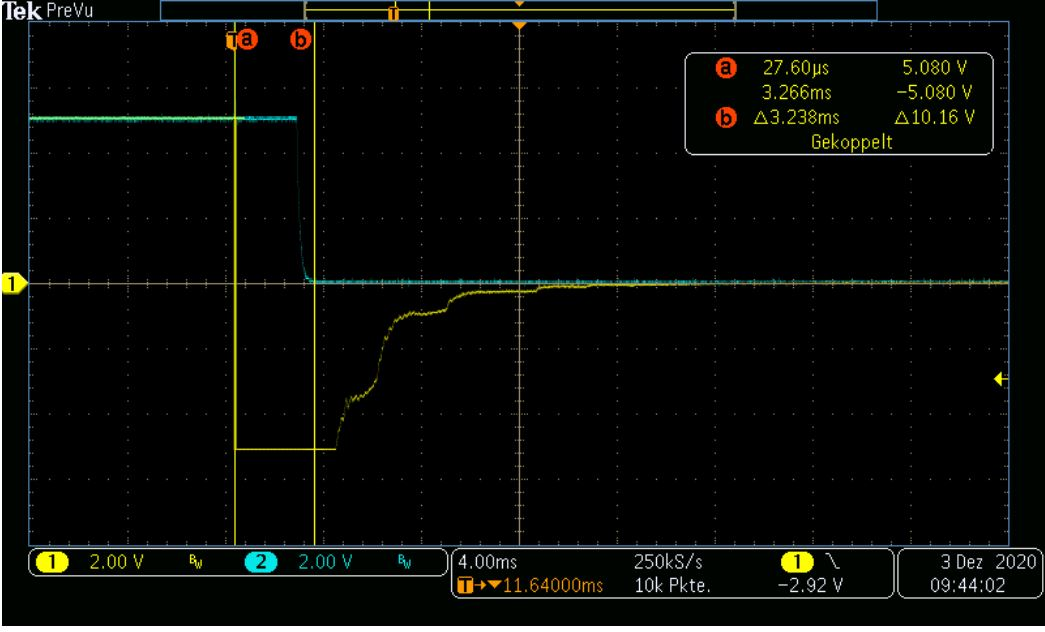
\includegraphics[scale=0.45]{../assets/images/ET2P4/aufgabe2c.JPG}
        \caption{Der Ausschaltvorgang ohne Freilaufdiode (ungelöscht)}
    \end{center}
\end{figure}
\newpage
\subsection{Ausschaltvorgang mit Freilaufdiode}

Wir wiederholen den vorhergegangen Versuch nun mit einer Freilaufdiode (eingebaut wie auf dem Schaltbild 2 in der Aufgabenstellung(s. oben)). Der Wert für $\hat{u}_{Rel} = 15V$ und $t_{aus} = 19,56ms$ werden 
ebenfalls aufgezeichnet.

\begin{figure}[!h]
  \begin{center}
    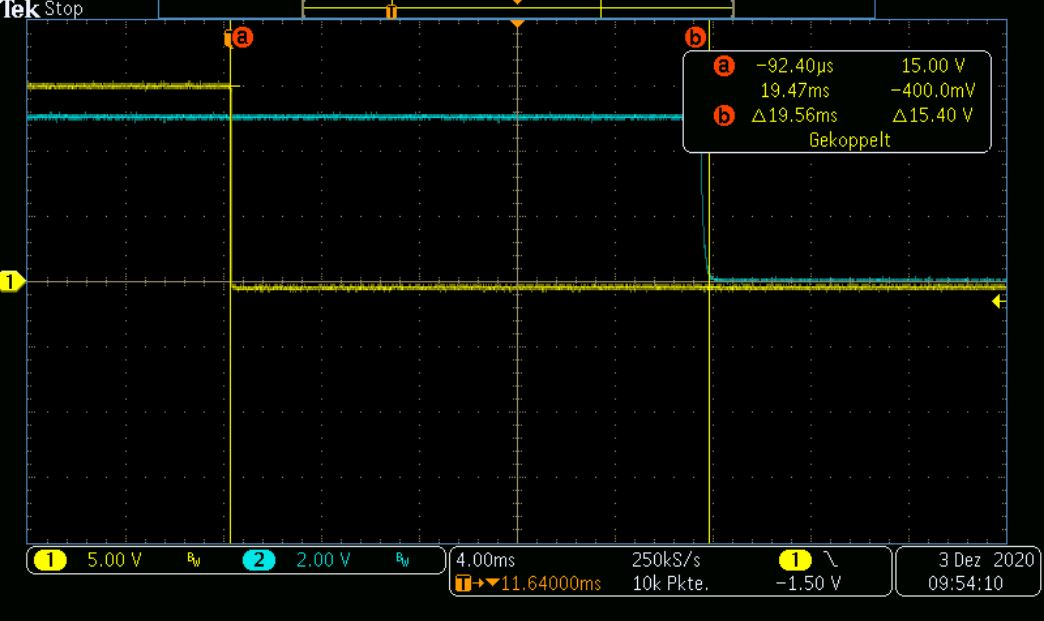
\includegraphics[scale=0.45]{../assets/images/ET2P4/aufgabe2d.JPG}
    \caption{Ausschaltvorgang mithilfe einer Freilaufdiode. Der Prozess wird länger jedoch offensichtlich kontrollierter}
  \end{center}
\end{figure}

\subsection{Bestimmung von Induktivität und Gleichstromwiderstand, sowie Ausschaltverzögerung}

Wir messen den Gleichstromwiderstand des Relais $R_{gl} = 863,6\Omega$ mithilfe des MetraHit Tech Multimeters.
\subsubsection{Ohne Freilaufdiode}

Wir wollen nun die Induktivität der Spule bestimmen, indem wir einen weiteren Einschaltvorgang simulieren und daraus die Zeitkonstante $\tau$ bestimmen. 
Aus der Zeitfunktion der Spule:
\begin{equation}
    I(t) = I_0 \cdot \left(1-e^{-\frac{R}{L}\cdot t}\right) 
\end{equation}
wissen wir, dass wir durch das Bestimmen von $\tau$ nun auch die Induktivität L über 
\begin{equation}\label{eq:Rt}
    L = R\cdot\tau
\end{equation}
berechnen können. Wir stellen dazu bei der Einschaltkurve der Spule die Cursorfunktion auf den Einschaltmoment und den Moment des Erreichens der 63\%-Grenze ein.
Wir erhalten damit ein $\tau = 13,48ms$. Mit (\ref{eq:Rt}) und dem Gleichstromwiderstand sowie dem Widerstand $R_M$ rechnen wir nun:
\begin{equation*}
    L = (R_M + R_{gl})\cdot \tau = (100\Omega + 863,6\Omega)\cdot 13,48ms = 12,988H
\end{equation*}

\newpage
\subsubsection{Mit Freilaufdiode}
\begin{figure}[h]
  \begin{center}
      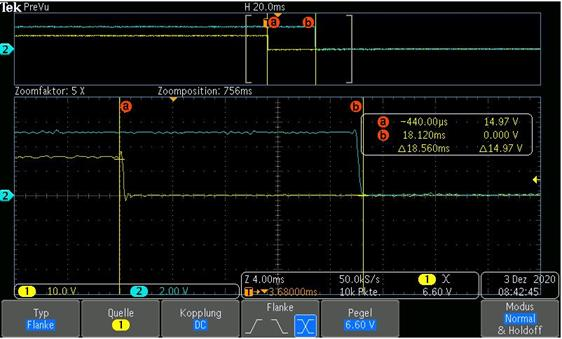
\includegraphics[scale=0.9]{../assets/images/ET2P4/mit freilaufdiode.jpg}
      \caption{Ausschaltvorgang mit Freilaufdiode}
  \end{center}
\end{figure}
Mittels der Cursor-Funktion wurde eine Abfallzeit t$_{ab}$ von 18ms ermittelt. Im Vergleich zur Schaltung ohne Freilaufdiode hat die Abfallzeit deutlich zugenommen.
Dafür kommt es jedoch zu keinen Spannungspitzen mehr.

\subsection{Auswertung}
Der Versuch hat relativ gut den Nutzen und die Funktionsweise eines Relais gezeigt. Dabei fungiert dies sozusagen als steuerbarer Schalter-.
Mittels einem Relais könnte man größere Lasten schalten, wobei das Relais selbst nur eine geringe Spannung benötigt. Sobald die Mindestspannung von 6,1V am Relais anliegt, zieht das Relais an und schließt damit den Schalter. Dieser Anzug ist auch leise zu hören.\\
Da das Relais eine induktive Last darstellt, kann beim Abschalten die in der Spule gespeicherte Energie unkontrolliert austreten. Beispielsweise durch kurze Spannungsspitzen, wodurch dann benachbarte elektrische Teile beschädigt werden können.
Wenn allerdings eine Diode parallel zum Relais und in Sperrrichtung zur Spannungsversorgung angeschlossen wird, wird die Energie in der Spule kontrolliert indem sich der Strom durch die Diode totläuft. 
Jedoch kommt es zu einer höheren Abfallzeit.

\newpage

\section{Auf- und Entladen eines Kondensators}
\begin{task}
TIn diesem Versuch geht es um den zeitlichen Verlauf einer Kondensatorspannung beim Auf- und Entladen. Betrachtet wird dabei der Zeitraum von etwa 5$\tau$.
\end{task}
\begin{figure}[h]
    \begin{center}
        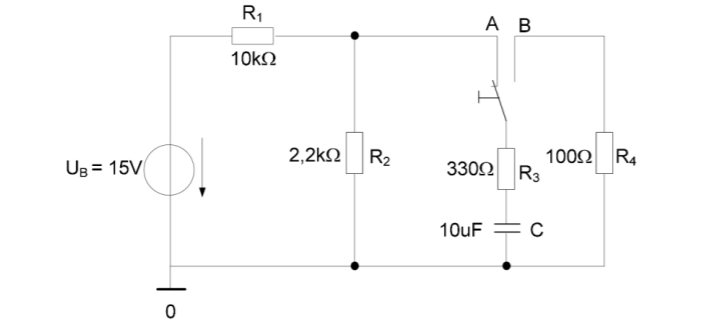
\includegraphics{../assets/images/ET2P4/Schaltplan3.PNG}
        \caption{Schaltplan der dritten Aufgabe mit jeweils zwei Schalterstellungen}
    \end{center}
\end{figure}

\begin{devlist}
    T
    \begin{itemize}
        \item Oszilloskop Tektronix MDO3012
        \item Funktionsgenerator Rhode \& Schwarz HM8150
    \end{itemize}
\end{devlist}
\newpage

\subsection{Aufladung, Schalterstellung A}
Berechnung der Aufladezeitkonsante und der Kondensatorspannung im aufgeladenen Zustand:
\begin{align*}
    \tau_A &= R\cdot C = (330\Omega + \left(\frac{1}{10k\Omega}+\frac{1}{2,2k\Omega}\right)^{-1}) \cdot 10\mu F\\
    \tau_A &= 21,3ms\\\\
    U_c &= U_{R2} = U_B \cdot \left(\frac{R2}{R1+R2}\right) = 15V \cdot \left(\frac{2,2k\Omega}{10k\Omega+2,2k\Omega}\right)\\
    U_c &= 2,7V
\end{align*}
Für den Aufladevorgang lautet die Funktion u$_c$(t) lautet dann:
\begin{align*}
    u_c(t)&= U_0 \cdot (1 - e^{-\frac{t}{RC}})\\
    u_c(t)&= 2,7V \cdot (1 - e^{-\frac{t}{21,3ms}})
\end{align*}
\begin{figure}[h]
  \begin{center}
    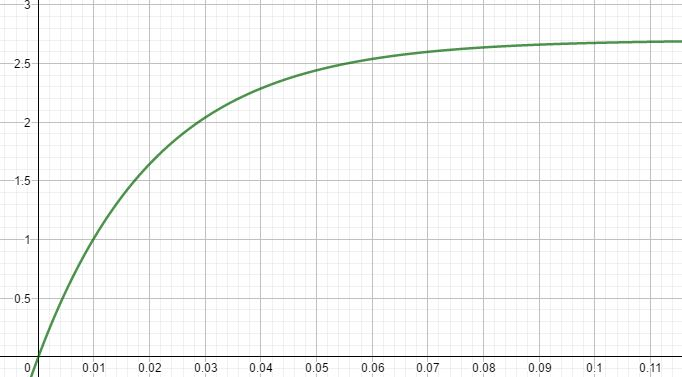
\includegraphics[scale=0.6]{../assets/images/ET2P4/aufladefunktion.JPG}
    \caption{Aufladefunktion des Kondensator mit Matlab simuliert}
  \end{center}
\end{figure}

 
\newpage
\subsection{Entladung, Schalterstellung B}
Berechnung der Entladezeitkonstante $\tau_E$:
\begin{align*}
    \tau_E &= R\cdot C = (330\Omega + 100\Omega) \cdot 10\mu F \\
    \tau_E &= 4300\mu s = 4,3ms
\end{align*}
Die dazugehörige Entladefunktion u$_c$(t) lautet:
\begin{align*}
    u_c(t)&= U_0 \cdot e^{-\frac{t}{RC}}\\
    u_c(t)&= 2,7V \cdot e^{-\frac{t}{4,3ms}}
\end{align*}

\begin{figure}[h]
  \begin{center}
    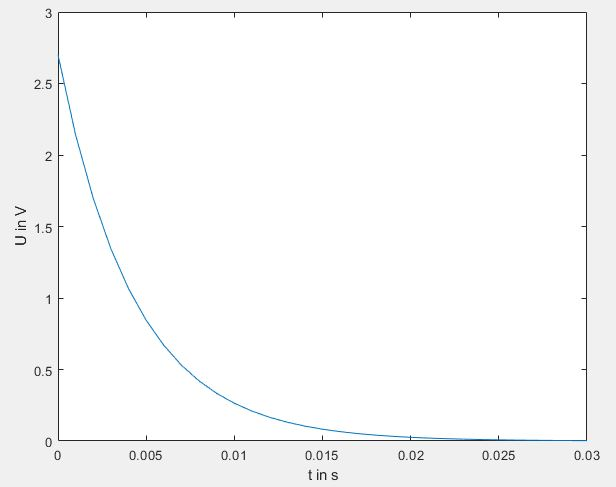
\includegraphics[scale=0.6]{../assets/images/ET2P4/entladefunktion.JPG}
    \caption{Entladefunktion des Kondensator mit Matlab simuliert}
  \end{center}
\end{figure}

\newpage
\subsection{Messung mit Oszilloskop}

\begin{figure}[h!]
  \begin{center}
    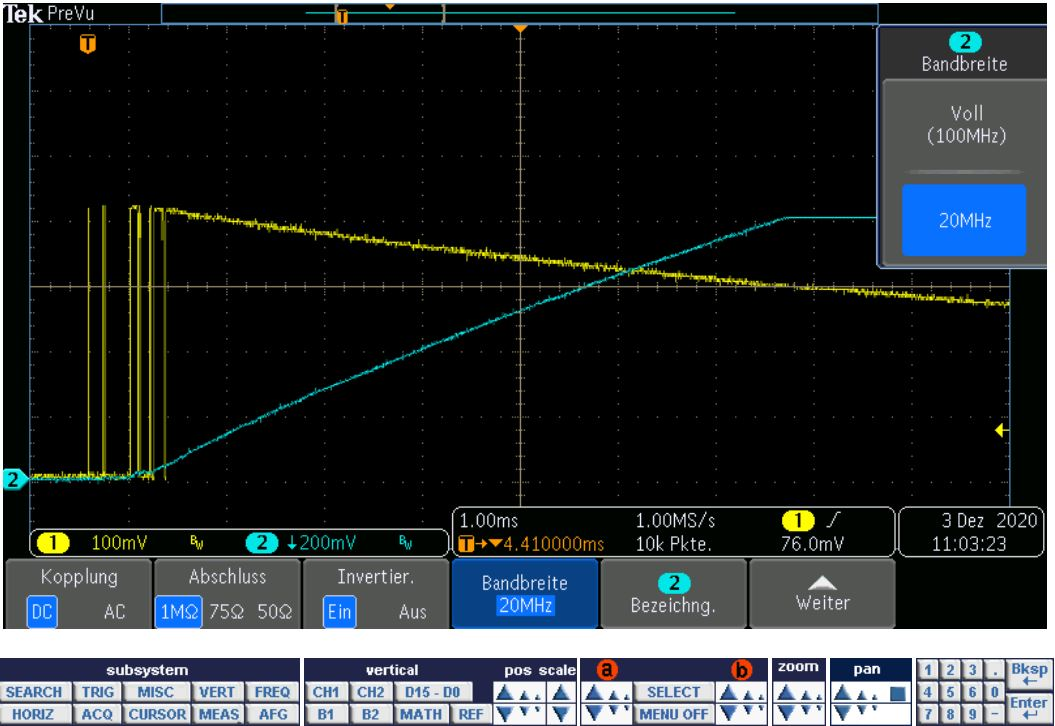
\includegraphics[scale=0.45]{../assets/images/ET2P4/aufgabe3Fehler.JPG}
    \caption{Fehlerhaftes Verhalten der Ladekurve des Kondensators durch unzureichendes Einstellen des Oszilloskops}
    \label{fig:error}
  \end{center}
\end{figure}

Im Zuge unsere Messung der tatsächlichen Auf- und Entladefunktion sind uns einige grundlegende Fehler unterlaufen. Wie auf der Abbildung (\ref{fig:error}) zu 
sehen, haben wir eine Ladekurve, die von zwei $\tau$ bestimmt zu sein scheint. Ein langsam steigendes $\tau_1$, welches die Kurve annähernd linear macht und ein 
$\tau_2$, welches ein abruptes (sehr schnelles) Ende der Ladekurve bestimmt, welches als scharfe Ecke erkannt wird. Diese Fehler entstanden durch ein fehlerhaftes Einstellen des Maßstabes am
Oszilloskop. Wir haben in einer Weise nur einen kleinen Teil der Ladekurve betrachtet und haben daher diese sehr befremdlich anmutende Kurve bekommen. Das Oszilloskop versucht hier den 
kompletten Verlauf abzubilden, stellt den ersten Verlauf daher als linear, also sehr schwach steigend dar. Ab einem Punkt muss der Prozess jedoch abgebrochen werden, da die Speicherkapazitäten überschritten werden.
Es kommt zu einer schnellen Beendigung des Prozesses.
Darüberhinaus nehmen die Schwingungen am Einschaltpunkt der Aufnahme ihren Ursprung in der Schwingung des verwendeten Schalters und der rauen Oberfläche der Schalterflächen, die an ihren Spitzen Kontakt aufbauen, dann jedoch
durch die Hitze schmelzen und den Kontakt erneut abbrechen.


\end{document}
